\chapter{Vector Spaces}


\section{Vector Space}

\begin{enumerate}
    \item \textbf{Definition}: A real-valued vector space $V = (\mathcal{V}, +, \cdot)$ is a set $\mathcal{V}$ with two operations:
    \hfill \cite{mfml/book/mml/Deisenroth-Faisal-Ong}
    \begin{enumerate}
        \item[] $+ :  \mathcal{V} \times \mathcal{V} \to \mathcal{V}$
        \hfill \cite{mfml/book/mml/Deisenroth-Faisal-Ong}

        \item[] $\cdot: \mathbb{R} \times \mathcal{V} \to \mathcal{V}$ 
        \hfill \cite{mfml/book/mml/Deisenroth-Faisal-Ong}
    \end{enumerate}


    \item addition ($+$) is inner operation: both operands must be from $\mathcal{V}$
    \hfill \cite{mfml/book/mml/Deisenroth-Faisal-Ong}

    \item multiplication by scalars ($\cdot$) is outer operation: one operand is from $\mathcal{V}$, another from $\mathbb{R}$
    \hfill \cite{mfml/book/mml/Deisenroth-Faisal-Ong}

    \item The elements $\bm{x} \in \mathcal{V}$ are called \textbf{vectors}.
    \hfill \cite{mfml/book/mml/Deisenroth-Faisal-Ong}
\end{enumerate}


\subsection{Properties of a vector Space}

\begin{enumerate}
    \item $(\mathcal{V}, +)$ is an Abelian group
    \hfill \cite{mfml/book/mml/Deisenroth-Faisal-Ong}

    \item Distributivity:
    \begin{enumerate}
        \item $\forall \lambda  \in  \mathbb{R}, \bm{x}, \bm{y} \in  \mathcal{V} : \lambda  \cdot  (\bm{x} + \bm{y}) = \lambda  \cdot  \bm{x} + \lambda  \cdot  \bm{y}$
        \hfill \cite{mfml/book/mml/Deisenroth-Faisal-Ong}

        \item $\forall \lambda , \psi  \in  \mathbb{R}, \bm{x} \in  \mathcal{V} : (\lambda  + \psi ) \cdot  \bm{x} = \lambda  \cdot  \bm{x} + \psi  \cdot  \bm{x}$
        \hfill \cite{mfml/book/mml/Deisenroth-Faisal-Ong}
    \end{enumerate}

    \item Associativity (outer operation): $\forall \lambda , \psi  \in  \mathbb{R}, \bm{x} \in  \mathcal{V} : \lambda \cdot (\psi \cdot x) = (\lambda \psi )\cdot \bm{x}$
    \hfill \cite{mfml/book/mml/Deisenroth-Faisal-Ong}

    \item Neutral element with respect to the outer operation: $\forall \bm{x} \in  \mathcal{V} : 1\cdot \bm{x} = \bm{x}$
    \hfill \cite{mfml/book/mml/Deisenroth-Faisal-Ong}

    \item The neutral element of $(\mathcal{V}, +)$ is the zero vector $\bm{0} = [0, \cdots , 0]^\top$
    \hfill \cite{mfml/book/mml/Deisenroth-Faisal-Ong}

    \item A “vector multiplication” $\bm{ab}, \bm{a}, \bm{b} \in \mathbb{R}^n$, is \textbf{not defined}.
    \hfill \cite{mfml/book/mml/Deisenroth-Faisal-Ong}
\end{enumerate}


\subsection{Dimension of a vector Space}


\begin{enumerate}
    \item the dimension of $V$ is the number of basis vectors of $V$ , and we write $\dim(V)$.
    \hfill \cite{mfml/book/mml/Deisenroth-Faisal-Ong}

    \item The dimension of a vector space corresponds to the number of its basis vectors.
    \hfill \cite{mfml/book/mml/Deisenroth-Faisal-Ong}

    \item Intuitively, the dimension of a vector space can be thought of as the number of independent directions in this vector space.
    \hfill \cite{mfml/book/mml/Deisenroth-Faisal-Ong}

    \item The dimension of a vector space is not necessarily the number of elements in a vector. 
    For instance, the vector space $V = \text{span}[\begin{bmatrix}0 \\ 1\end{bmatrix}]$ is one-dimensional, although the basis vector possesses two elements.
    \hfill \cite{mfml/book/mml/Deisenroth-Faisal-Ong}
\end{enumerate}


\subsection{Norm}

\begin{enumerate}
    \item \textbf{Definition}: A norm on a vector space $V$ is a function
    \hfill \cite{mfml/book/mml/Deisenroth-Faisal-Ong}
    \\
    .\hfill
    $\dnorm{\cdot}: V \to \mathbb{R}$ such that $\bm{x} \mapsto \dnorm{\bm{x}}$
    \hfill \cite{mfml/book/mml/Deisenroth-Faisal-Ong}
    \\
    which assigns each vector $\bm{x}$ its length $\dnorm{\bm{x}} \in \mathbb{R}$, such that for all $\lambda \in \mathbb{R}$ and $\bm{x}, \bm{y} \in V$ the following hold:
    \hfill \cite{mfml/book/mml/Deisenroth-Faisal-Ong}
    \begin{enumerate}
        \item Absolutely homogeneous: $\dnorm{\lambda \bm{x}} = \dabs{\lambda} \dnorm{\bm{x}}$
        \hfill \cite{mfml/book/mml/Deisenroth-Faisal-Ong}

        \item Triangle inequality: $\dnorm{\bm{x} + \bm{y}} \leq \dnorm{\bm{x}} + \dnorm{\bm{y}}$
        \hfill \cite{mfml/book/mml/Deisenroth-Faisal-Ong}
        \\
        In geometric terms, the triangle inequality states that for any triangle, the sum of the lengths of any two sides must be greater than or equal to the length of the remaining side.
        

        \item Positive definite: $\dnorm{\bm{x}} \geq 0$ and $\dnorm{\bm{x}} = 0 \Leftrightarrow \bm{x} = \bm{0}$
        \hfill \cite{mfml/book/mml/Deisenroth-Faisal-Ong}
    \end{enumerate}
\end{enumerate}




\subsection{Inner Product Space}

\begin{enumerate}
    \item Let $V$ be a vector space and $\Omega  : V \times  V \to  \mathbb{R}$ be a bilinear mapping that takes two vectors and maps them onto a real number. 
    Then the pair $(V, \dAngleBrac{\cdot, \cdot})$ is called an \textbf{inner product space} or \textbf{(real) vector space with inner product}.
\end{enumerate}




\subsection{Euclidean vector space}

\begin{enumerate}
    \item Let $V$ be a vector space and $\Omega : V \times V \to \mathbb{R}$ be a bilinear mapping that takes two vectors and maps them onto a real number. Then if we use the dot product, we call $(V,\dAngleBrac{\cdot, \cdot})$ a Euclidean vector space.
\end{enumerate}



\subsection{Lengths}

\begin{enumerate}
    \item Inner products and norms are closely related in the sense that any inner product induces a norm
    \hfill \cite{mfml/book/mml/Deisenroth-Faisal-Ong}
    \\
    .\hfill
    $\dnorm{\bm{x}} := \sqrt{\dAngleBrac{\bm{x}, \bm{x}}}$
    \hfill \cite{mfml/book/mml/Deisenroth-Faisal-Ong}
    \\
    in a natural way, such that we can compute lengths of vectors using the inner product.
    \hfill \cite{mfml/book/mml/Deisenroth-Faisal-Ong}

    \item length = norm
    \hfill \cite{common/online/chatgpt}
    \\
    different norms lead to different lengths
    \hfill \cite{common/online/chatgpt}

    \item Not every norm is induced by an inner product (eg: Manhattan norm).
    \hfill \cite{mfml/book/mml/Deisenroth-Faisal-Ong}

    \item \textbf{Cauchy-Schwarz Inequality}: For an inner product vector space $(V,\dAngleBrac{\cdot, \cdot})$ the induced norm $\dnorm{\cdot}$ satisfies the Cauchy-Schwarz inequality
    \hfill \cite{mfml/book/mml/Deisenroth-Faisal-Ong}
    \\
    .\hfill
    $\dabs{\dAngleBrac{\bm{x}, \bm{y}}} \leq \dnorm{\bm{x}} \dnorm{\bm{y}}$
    \hfill \cite{mfml/book/mml/Deisenroth-Faisal-Ong}

    \item Transformations by orthogonal matrices are special because the length of a vector $\bm{x}$ is not changed when transforming it using an orthogonal matrix $\bm{A}$. 
    For the dot product, we obtain
    \hfill \cite{mfml/book/mml/Deisenroth-Faisal-Ong}
    \\
    .\hfill
    $
        \dnorm{\bm{Ax}}^2 
        = (\bm{Ax})^\top (\bm{Ax})
        = \bm{x}^\top \bm{A}^\top \bm{Ax}
        = \bm{x}^\top \bm{Ix}
        = \bm{x}^\top \bm{x}
        = \dnorm{\bm{x}}^2
    $
    \hfill \cite{mfml/book/mml/Deisenroth-Faisal-Ong}
\end{enumerate}





\subsection{Distance}

\begin{enumerate}
    \item Consider an inner product space $(V,\dAngleBrac{\cdot, \cdot})$. 
    Then
    \hfill \cite{mfml/book/mml/Deisenroth-Faisal-Ong}
    \\
    .\hfill
    $
        d(\bm{x}, \bm{y})
        := \dnorm{\bm{x} - \bm{y}}
        = \sqrt{\dAngleBrac{\bm{x} - \bm{y}, \bm{x} - \bm{y}}}
    $
    \hfill \cite{mfml/book/mml/Deisenroth-Faisal-Ong}
    \\
    is called the distance between $\bm{x}$ and $\bm{y}$ for $\bm{x}, \bm{y} \in V$ .
    \hfill \cite{mfml/book/mml/Deisenroth-Faisal-Ong}

    \item If we use the dot product as the inner product, then the distance is called \textbf{Euclidean distance}.
    \hfill \cite{mfml/book/mml/Deisenroth-Faisal-Ong}

    \item Similar to the length of a vector, the distance between vectors does not require an inner product: a norm is sufficient.
    If we have a norm induced by an inner product, the distance may vary depending on the choice of the inner product. 
    \hfill \cite{mfml/book/mml/Deisenroth-Faisal-Ong}

    \item Every distance is a metric, but not every metric is necessarily defined as a distance using a norm or inner product.
    \hfill \cite{common/online/chatgpt}

    \item \item Transformations with orthogonal matrices preserve distances.
    \hfill \cite{mfml/book/mml/Deisenroth-Faisal-Ong}
\end{enumerate}




\subsection{Metric}

\begin{enumerate}
    \item \textbf{Definition}: The mapping $d : V \times V \to \mathbb{R}$, $(\bm{x}, \bm{y}) \mapsto d(\bm{x}, \bm{y})$ is called a \textbf{metric}.
    \hfill \cite{mfml/book/mml/Deisenroth-Faisal-Ong}

    \item A metric $d$ satisfies the following:
    \hfill \cite{mfml/book/mml/Deisenroth-Faisal-Ong}
    \begin{enumerate}
        \item $d$ is \textbf{positive definite}, i.e., $d(\bm{x}, \bm{y}) \geq 0$ for all $\bm{x}, \bm{y} \in V$ and $d(\bm{x}, \bm{y}) = 0 \Leftrightarrow \bm{x} = \bm{y}$ .
        \hfill \cite{mfml/book/mml/Deisenroth-Faisal-Ong}

        \item $d$ is \textbf{symmetric}, i.e., $d(\bm{x}, \bm{y}) = d(\bm{y}, \bm{x})$ for all $\bm{x}, \bm{y} \in V$ .
        \hfill \cite{mfml/book/mml/Deisenroth-Faisal-Ong}

        \item \textbf{Triangle inequality}: $d(\bm{x}, \bm{z}) \leq d(\bm{x}, \bm{y}) + d(\bm{y}, \bm{z})$ for all $\bm{x}, \bm{y}, \bm{z} \in V$ .
        \hfill \cite{mfml/book/mml/Deisenroth-Faisal-Ong}
    \end{enumerate}
\end{enumerate}



\subsection{Inner Product VS Metric}

\begin{enumerate}
    \item the lists of properties of inner products and metrics look very similar. 
    \hfill \cite{mfml/book/mml/Deisenroth-Faisal-Ong}

    \item $\dAngleBrac{\bm{x}, \bm{y}}$ and $d(\bm{x}, \bm{y})$ behave in opposite directions.
    \hfill \cite{mfml/book/mml/Deisenroth-Faisal-Ong}

    \item Very similar $\bm{x}$ and $\bm{y}$ will result in a large value for the inner product and a small value for the metric.
    \hfill \cite{mfml/book/mml/Deisenroth-Faisal-Ong}
\end{enumerate}




\subsection{Angles}

\begin{enumerate}
    \item We use the Cauchy-Schwarz inequality to define angles $\omega$ in inner product spaces between two vectors $\bm{x}, \bm{y}$, and this notion coincides with our intuition in $\mathbb{R}^2$ and $\mathbb{R}^3$. 
    Assume that $\bm{x} \neq \bm{0}$, $\bm{y} \neq \bm{0}$. 
    Then
    $
        -1 \leq \dfrac{\dAngleBrac{\bm{x}, \bm{y}}}{\dnorm{\bm{x}} \dnorm{\bm{y}}} \leq 1
    $. 
    Therefore, there exists a unique $\omega \in [0, \pi]$ with 
    $
        \cos(\omega) = \dfrac{\dAngleBrac{\bm{x}, \bm{y}}}{\dnorm{\bm{x}} \dnorm{\bm{y}}}
    $
    \hfill \cite{mfml/book/mml/Deisenroth-Faisal-Ong}

    \item The number $\omega$ is the angle between the vectors $\bm{x}$ and $\bm{y}$.
    \hfill \cite{mfml/book/mml/Deisenroth-Faisal-Ong}

    \item Intuitively, the angle between two vectors tells us how similar their orientations are.
    \hfill \cite{mfml/book/mml/Deisenroth-Faisal-Ong}

    \item Transformations with orthogonal matrices preserve angles.
    \hfill \cite{mfml/book/mml/Deisenroth-Faisal-Ong}
    \\
    The angle between any two vectors $\bm{x}, \bm{y}$, as measured by their inner product, is also unchanged when transforming both of them using an orthogonal matrix $\bm{A}$. 
    Assuming the dot product as the inner product, the angle of the images $\bm{Ax}$ and $\bm{Ay}$ is given as
    \hfill \cite{mfml/book/mml/Deisenroth-Faisal-Ong}
    \\
    .\hfill
    $
        \cos \omega
        = \dfrac{(\bm{Ax})^\top (\bm{Ax})}{\dnorm{\bm{Ax}} \dnorm{\bm{Ax}}}
        = \dfrac{\bm{x}^\top \bm{A}^\top\bm{Ay}}{\sqrt{\bm{x}^\top \bm{A}^\top\bm{Ax} \bm{y}^\top \bm{A}^\top\bm{Ay}}}
        = \dfrac{\bm{x}^\top \bm{y}}{\dnorm{\bm{x}} \dnorm{\bm{y}}}
    $
    \hfill \cite{mfml/book/mml/Deisenroth-Faisal-Ong}
    \\
    which gives exactly the angle between $\bm{x}$ and $\bm{y}$.
\end{enumerate}

\begin{customArrayStretch}{1.3}
\begin{table}[H]
    \centering
    \begin{tabular}{|l|l|l|}
        \hline
        $\omega$ & $\cos(\omega)$ & Interpretation \\
        \hline
        $0$ & $1$ & orientation is same \\
        ${\pi}/{2}$ & $0$ & perpendicular \\
        $\pi$ & $-1$ & opposite direction \\
        \hline
    \end{tabular}
\end{table}
\end{customArrayStretch}




















\section{Vector Subspace/ linear subspace}


\begin{enumerate}
    \item \textbf{Definition}: Let $V = (\mathcal{V}, +, \cdot )$ be a vector space and $\mathcal{U} \subseteq \mathcal{V}, \mathcal{U} \neq \phi$. 
    Then $U = (\mathcal{U}, +, \cdot )$ is called vector subspace of $V$ (or linear subspace) if $U$ is a vector space with the vector space operations $+$ and $\cdot$  restricted to $\mathcal{U} \times \mathcal{U}$ and $\mathbb{R} \times \mathcal{U}$. 
    We write $U \subseteq V$ to denote a subspace $U$ of $V$.
    \hfill \cite{mfml/book/mml/Deisenroth-Faisal-Ong}

    \item Intuitively, they are sets contained in the original vector space with the property that when we perform vector space operations on elements within this subspace, we will never leave it. 
    In this sense, they are “closed”.
    \hfill \cite{mfml/book/mml/Deisenroth-Faisal-Ong}

    \item If $\mathcal{U} \subseteq \mathcal{V}$ and $V$ is a vector space, then $U$ naturally inherits many properties directly from $V$ because they hold for all $\bm{x} \in \mathcal{V}$, and in particular for all $\bm{x} \in \mathcal{U} \subseteq \mathcal{V}$. 
    This includes the Abelian group properties, the distributivity, the associativity and the neutral element.
    \hfill \cite{mfml/book/mml/Deisenroth-Faisal-Ong}

    \item To determine whether $(\mathcal{U}, +, \cdot)$ is a subspace of V we still do need to show:
    \begin{enumerate}
        \item $\mathcal{U} \neq \phi$, in particular: $\bm{0} \in \mathcal{U}$
        \hfill \cite{mfml/book/mml/Deisenroth-Faisal-Ong}

        \item Closure of $U$:
        \begin{enumerate}
            \item With respect to the outer operation: $\forall \lambda  \in  \mathbb{R} \forall \bm{x} \in  \mathcal{U} : \lambda \bm{x} \in  \mathcal{U}$.
            \hfill \cite{mfml/book/mml/Deisenroth-Faisal-Ong}
            
            \item With respect to the inner operation: $\forall \bm{x}, \bm{y} \in  \mathcal{U} : \bm{x} + \bm{y} \in  \mathcal{U}$.
            \hfill \cite{mfml/book/mml/Deisenroth-Faisal-Ong}
        \end{enumerate}
    \end{enumerate}

\end{enumerate}


\subsection{Dimension of a Vector Subspace}

\begin{enumerate}
    \item If $U \subseteq V$ is a subspace of $V$ , then $\dim(U) \leq \dim(V )$ and $\dim(U) = \dim(V )$ if and only if $U = V$ .
    \hfill \cite{mfml/book/mml/Deisenroth-Faisal-Ong}
\end{enumerate}



\subsection{Basis of a Vector Subspace}

\begin{enumerate}
    \item A basis of a subspace $U = \text{span}[\bm{x}_1, \cdots , \bm{x}_m] \subseteq \mathbb{R}^n$ can be found by executing the following steps:
    \hfill \cite{mfml/book/mml/Deisenroth-Faisal-Ong}
    \begin{enumerate}
        \item Write the spanning vectors as columns of a matrix $\bm{A}$
        \hfill \cite{mfml/book/mml/Deisenroth-Faisal-Ong}

        \item Determine the row-echelon form (REF) of $\bm{A}$.
        \hfill \cite{mfml/book/mml/Deisenroth-Faisal-Ong}

        \item The spanning vectors associated with the pivot columns are a basis of $U$.
        \hfill \cite{mfml/book/mml/Deisenroth-Faisal-Ong}
    \end{enumerate}
\end{enumerate}
























\section{Vector}

\begin{enumerate}
    \item In general, vectors are special objects that can be added together and multiplied by scalars to produce another object of the same kind. From an abstract mathematical viewpoint, any object that satisfies these two properties can be considered a vector. 
    \hfill \cite{mfml/book/mml/Deisenroth-Faisal-Ong}

    \item By convention $(1, n)$-matrices are called rows and $(m, 1)$-matrices are called row columns. 
    These special matrices are also called row/ column vectors.
    \hfill \cite{mfml/book/mml/Deisenroth-Faisal-Ong}

    \item Geometric vectors directed line segments that start at the origin, then intuitively the length of a vector is the distance of the “end” of this directed line segment from the origin.
    \hfill \cite{mfml/book/mml/Deisenroth-Faisal-Ong}
\end{enumerate}




\subsection{Types of vectors}

\begin{enumerate}
    \item $\mathbb{R}^n$ or $\mathbb{R}^{n\times 1}$ : column vectors: 
    $
        \bm{x} = 
        \begin{bmatrix}
            x_1\\ \vdots \\ x_n
        \end{bmatrix}
    $
    \hfill \cite{mfml/book/mml/Deisenroth-Faisal-Ong}

    \item $\mathbb{R}^{1\times n}$ : row vectors: 
    $
        \bm{x}^\top = \begin{bmatrix}x_1 & \cdots & x_n\end{bmatrix}
    $
    \hfill \cite{mfml/book/mml/Deisenroth-Faisal-Ong}
\end{enumerate}






\subsection{Manhattan Norm/ $\ell_1$ Norm}

\begin{enumerate}
    \item The Manhattan norm on $\mathbb{R}^n$ is defined for $\bm{x} \in \mathbb{R}^n$ as
    \hfill \cite{mfml/book/mml/Deisenroth-Faisal-Ong}
    \\
    .\hfill
    $
        \dnorm{\bm{x}}_1 := \dsum^n_{i=1} \dabs{x_i}
    $
    \hfill \cite{mfml/book/mml/Deisenroth-Faisal-Ong}
    \\
    where $\dabs{\cdot}$ is the absolute value.
    \hfill \cite{mfml/book/mml/Deisenroth-Faisal-Ong}
\end{enumerate}



\subsection{Euclidean Norm/ $\ell_2$ Norm}

\begin{enumerate}
    \item The Euclidean norm of $\bm{x} \in \mathbb{R}^n$ is defined as
    \hfill \cite{mfml/book/mml/Deisenroth-Faisal-Ong}
    \\
    .\hfill
    $
        \dnorm{\bm{x}}_2 := \sqrt{ \dsum^n_{i=1} x_i^2 } = \sqrt{\bm{x}^\top\bm{x}}
    $
    \hfill \cite{mfml/book/mml/Deisenroth-Faisal-Ong}
    \\
    and computes the Euclidean distance of $\bm{x}$ from the origin.
    \hfill \cite{mfml/book/mml/Deisenroth-Faisal-Ong}

    \item default "norm", if not stated otherwise.
    \hfill \cite{mfml/book/mml/Deisenroth-Faisal-Ong}
\end{enumerate}



\subsection{Outer Product ($ab^\top$) }

\begin{enumerate}
    \item $\forall \bm{a}, \bm{b} \in \mathbb{R}^n, \bm{ab}^\top \in \mathbb{R}^{n\times n}$
    \hfill \cite{mfml/book/mml/Deisenroth-Faisal-Ong}
    
\end{enumerate}



\subsection{General Inner Product ( $\Omega(a, b)$ )}

\begin{enumerate}
    \item A bilinear mapping $\Omega$ is a mapping with two arguments, and it is linear in each argument, i.e., when we look at a vector space $V$ then it holds that for all $\bm{x}, \bm{y}, \bm{z} \in V, \lambda , \psi  \in \mathbb{R}$ that
    \hfill \cite{mfml/book/mml/Deisenroth-Faisal-Ong}
    \\
    .\hfill
    $\Omega(\lambda \bm{x} + \psi \bm{y}, \bm{z}) = \lambda \Omega(\bm{x}, \bm{z}) + \psi \Omega(\bm{y}, \bm{z})$
    \hfill \cite{mfml/book/mml/Deisenroth-Faisal-Ong}
    \\
    .\hfill
    $\Omega(\bm{x}, \lambda \bm{y} + \psi \bm{z}) = \lambda \Omega(\bm{x}, \bm{y}) + \psi \Omega(\bm{x}, \bm{z})$.
    \hfill \cite{mfml/book/mml/Deisenroth-Faisal-Ong}

    \item Let $V$ be a vector space and $\Omega : V \times  V \to \mathbb{R}$ be a bilinear mapping that takes two vectors and maps them onto a real number. Then
    \hfill \cite{mfml/book/mml/Deisenroth-Faisal-Ong}
    \begin{enumerate}
        \item $\Omega$ is called \textbf{symmetric} if $\Omega(\bm{x}, \bm{y}) = \Omega(\bm{y}, \bm{x})$ for all $\bm{x}, \bm{y} \in  V$ , i.e., the order of the arguments does not matter.
        \hfill \cite{mfml/book/mml/Deisenroth-Faisal-Ong}

        \item $\Omega$ is called \textbf{positive definite} if $\forall \bm{x} \in  V \backslash \dCurlyBrac{\bm{0}} : \Omega(\bm{x}, \bm{x}) > 0 , \Omega(\bm{0}, \bm{0}) = 0$.
        \hfill \cite{mfml/book/mml/Deisenroth-Faisal-Ong}
    \end{enumerate}

\end{enumerate}





\subsection{Inner Product ( $<x, y>$ )}

\begin{enumerate}
    \item Let $V$ be a vector space and $\Omega  : V \times  V \to  \mathbb{R}$ be a bilinear mapping that takes two vectors and maps them onto a real number. Then
    \begin{enumerate}
        \item A positive definite, symmetric bilinear mapping $\Omega  : V \times  V \to  \mathbb{R}$ is called an inner product on $V$ . 
        We typically write $\dAngleBrac{x, y}$ instead of $\Omega (x, y)$.        
    \end{enumerate}
\end{enumerate}





\subsection{Scalar/dot product ($a^\top b$)}


\begin{enumerate}
    \item $
        \forall \bm{a}, \bm{b} \in \mathbb{R}^n, 
        \bm{a}^\top \bm{b} = \dsum^n_{i=1} a_i b_i \in \mathbb{R}    
    $
    \hfill \cite{mfml/book/mml/Deisenroth-Faisal-Ong}
    
\end{enumerate}



\subsection{Orthogonal ( $x \perp y$ ) \& orthonormal vectors}

\begin{enumerate}
    \item \textbf{Definition}: Two vectors $\bm{x}$ and $\bm{y}$ are orthogonal if and only if $\dAngleBrac{\bm{x}, \bm{y}} = 0$, and we write $\bm{x} \perp \bm{y}$. 
    \hfill \cite{mfml/book/mml/Deisenroth-Faisal-Ong}
    
    \item If additionally $\dnorm{\bm{x}} = 1 = \dnorm{\bm{y}}$, i.e., the vectors are unit vectors, then $\bm{x}$ and $\bm{y}$ are orthonormal.
    \hfill \cite{mfml/book/mml/Deisenroth-Faisal-Ong}

    \item $\bm{0}$-vector is orthogonal to every vector in the vector space.
    \hfill \cite{mfml/book/mml/Deisenroth-Faisal-Ong}

    \item Orthogonality is the generalization of the concept of perpendicularity to bilinear forms that do not have to be the dot product.
    \hfill \cite{mfml/book/mml/Deisenroth-Faisal-Ong}
\end{enumerate}



























\section{Linear Combination}

\begin{enumerate}
    \item \textbf{Definition}: Consider a vector space $V$ and a finite number of vectors $\bm{x}_1, \cdots , \bm{x}_k \in V$ . 
    Then, every $\bm{v} \in V$ of the form:
    \\
    .\hfill
    $
        \bm{v} 
        = \lambda _1 \bm{x}_1 + \cdots + \lambda _k \bm{x}_k
        = \dsum_{i=1}^k \lambda _i \bm{x}_i
        \in V
    $
    \hfill.
    \\
    with $\lambda _1, \cdots , \lambda _k \in \mathbb{R}$ is a linear combination of the vectors $\bm{x}_1, \cdots , \bm{x}_k$.
    \hfill \cite{mfml/book/mml/Deisenroth-Faisal-Ong}

    \item The $\bm{0}$-vector can always be written as the linear combination of $k$ vectors $\bm{x}_1, \cdots , \bm{x}_k$ because $\bm{0} = \dsum ^k _{i=1} 0 \bm{x}_i$ is always true.
    \hfill \cite{mfml/book/mml/Deisenroth-Faisal-Ong}

    
\end{enumerate}







\section{Affine Subspaces}

\begin{enumerate}
    \item \textbf{Definition}: Let $V$ be a vector space, $\bm{x}_0 \in V$ and $U \subseteq V$ a subspace. 
    Then the subset 
    \hfill \cite{mfml/book/mml/Deisenroth-Faisal-Ong}
    \\
    .\hfill
    $
        L 
        = \bm{x}_0 + U 
        := \dCurlyBrac{\bm{x}_0 + \bm{u} : \bm{u} \in  U}
        = \dCurlyBrac{\bm{v} \in  V | \exists \bm{u} \in  U : \bm{v} = \bm{x}_0 + \bm{u}} \subseteq V
    $
    \hfill \cite{mfml/book/mml/Deisenroth-Faisal-Ong}
    \\
    is called \textbf{affine subspace} or \textbf{linear manifold} of $V$.
    $U$ is called \textbf{direction} or \textbf{direction space}, and $\bm{x}_0$ is called \textbf{support point}.
    $L$ is also known as \textbf{hyperplane}.
    \hfill \cite{mfml/book/mml/Deisenroth-Faisal-Ong}

    \item Note that the definition of an affine subspace excludes $\bm{0}$ if $\bm{x}_0 \notin U$.
    Therefore, an affine subspace is not a (linear) subspace (vector subspace) of $V$ for $\bm{x}_0 \notin U$.
    \hfill \cite{mfml/book/mml/Deisenroth-Faisal-Ong}

    \item Consider two affine subspaces $L = \bm{x}_0 + U$ and $\tilde{L} = \tilde{\bm{x}}_0 + \tilde{U}$ of a vector space $V$ . 
    Then, $L \subseteq \tilde{L}$ if and only if $U \subseteq \tilde{U}$ and $\bm{x}_0 - \tilde{\bm{x}}_0 \in \tilde{U}$.
    \hfill \cite{mfml/book/mml/Deisenroth-Faisal-Ong}

    \item Affine subspaces are often described by parameters: Consider a $k$-dimensional affine space $L = \bm{x}_0 + U$ of $V$ . 
    If $(\bm{b}_1, \cdots , \bm{b}_k)$ is an ordered basis of $U$, then every element $\bm{x} \in L$ can be uniquely described as
    \hfill \cite{mfml/book/mml/Deisenroth-Faisal-Ong}
    \\
    .\hfill
    $
        \bm{x} = \bm{x}_0 + \lambda _1 \bm{b}_1 + \cdots + \lambda _k \bm{b}_k
    $
    \hfill \cite{mfml/book/mml/Deisenroth-Faisal-Ong}
    \\
    where $\lambda _1, \cdots , \lambda _k \in \mathbb{R}$. 
    This representation is called parametric equation of $L$ with directional vectors $\bm{b}_1, \cdots , \bm{b}_k$ and parameters $\lambda _1, \cdots , \lambda _k$.
    \hfill \cite{mfml/book/mml/Deisenroth-Faisal-Ong}

    \item One-dimensional affine subspaces are called \textbf{lines} and can be written as $\bm{y} = \bm{x}_0 + \lambda \bm{b}_1$, where $\lambda  \in \mathbb{R}$ and $U = \text{span}[\bm{b}_1] \subseteq \mathbb{R}^n$ is a one-dimensional subspace of $\mathbb{R}^n$ . 
    This means that a line is defined by a support point $\bm{x}_0$ and a vector $\bm{b}_1$ that defines the direction.
    \hfill \cite{mfml/book/mml/Deisenroth-Faisal-Ong}

    \item Two-dimensional affine subspaces of $\bm{R}^n$ are called \textbf{planes}. 
    The parametric equation for planes is $\bm{y} = \bm{x}_0 + \lambda _1 \bm{b}_1 + \lambda _2 \bm{b}_2$, where $\lambda _1, \lambda _2 \in \mathbb{R}$ and $U = \text{span}[\bm{b}_1, \bm{b}_2] \subseteq \mathbb{R}^n$ . 
    This means that a plane is defined by a support point $\bm{x}_0$ and two linearly independent vectors $\bm{b}_1, \bm{b}_2$ that span the direction space.
    \hfill \cite{mfml/book/mml/Deisenroth-Faisal-Ong}

    \item In $\mathbb{R}^n$, the $(n - 1)$-dimensional affine subspaces are called \textbf{hyperplanes}, and the corresponding parametric equation is $\bm{y} = \bm{x}_0 + \dsum^ {n-1} _{i=1} \lambda_i \bm{b}_i$ , where $\bm{b}_1, \cdots , \bm{b}_{n-1}$ form a basis of an $(n - 1)$-dimensional subspace $U$ of $\mathbb{R}^n$ . 
    This means that a hyperplane is defined by a support point $\bm{x}_0$ and $(n - 1)$ linearly independent vectors $\bm{b}_1, \cdots , \bm{b}_{n-1}$ that span the direction space. 
    In $\mathbb{R}^2$ , a line is also a hyperplane. 
    In $\mathbb{R}^3$ , a plane is also a hyperplane.
    \hfill \cite{mfml/book/mml/Deisenroth-Faisal-Ong}

    
\end{enumerate}

















\section{Linear (In)dependence}

\begin{enumerate}
    \item \textbf{Definition}: Let us consider a vector space $V$ with $k \in \mathbb{N}$ and $\bm{x}_1, \cdots , \bm{x}_k \in V$ . 
    If there is a non-trivial linear combination, such that $\bm{0} = \dsum ^k _{i=1} \lambda_i \bm{x}_i$ with at least one $\lambda _i \neq 0$, the vectors  $\bm{x}_1, \cdots , \bm{x}_k$ are linearly dependent. 
    \hfill \cite{mfml/book/mml/Deisenroth-Faisal-Ong}
    
    \item If only the trivial solution exists, i.e., $\lambda _1 = \cdots = \lambda _k = 0$ the vectors $\bm{x}_1, \cdots , \bm{x}_k$ are linearly independent.
    \hfill \cite{mfml/book/mml/Deisenroth-Faisal-Ong}

    \item Intuitively, a set of linearly independent vectors consists of vectors that have no redundancy, i.e., if we remove any of those vectors from the set, we will lose something.
    \hfill \cite{mfml/book/mml/Deisenroth-Faisal-Ong}
\end{enumerate}


\subsection{Properties of Linear (In)dependence}
\begin{enumerate}
    \item $k$ vectors are either linearly dependent or linearly independent. There is no third option.
    \hfill \cite{mfml/book/mml/Deisenroth-Faisal-Ong}

    \item If at least one of the vectors $\bm{x}_1, \cdots , \bm{x}_k$ is $\bm{0}$ then they are linearly dependent. 
    The same holds if two vectors are identical.
    \hfill \cite{mfml/book/mml/Deisenroth-Faisal-Ong}

    \item The vectors $\dCurlyBrac{\bm{x}_1, \cdots , \bm{x}_k : \bm{x}_i \neq 0, i = 1, \cdots , k}$, $k \geq 2$, are linearly dependent if and only if (at least) one of them is a linear combination of the others. 
    In particular, if one vector is a multiple of another vector, i.e., $\bm{x}_i = \lambda \bm{x}_j , \lambda \in \mathbb{R}$ then the set $\dCurlyBrac{\bm{x}_1, \cdots , \bm{x}_k : \bm{x}_i \neq \bm{0}, i = 1, \cdots , k}$ is linearly dependent.
    \hfill \cite{mfml/book/mml/Deisenroth-Faisal-Ong}

    \item A practical way of checking whether vectors $\bm{x}_1, \cdots , \bm{x}_k \in V$ are linearly independent is to use Gaussian elimination: 
    Write all vectors as columns of a matrix $A$ and perform Gaussian elimination until the matrix is in row echelon form (the reduced row-echelon form is unnecessary here):
    \hfill \cite{mfml/book/mml/Deisenroth-Faisal-Ong}
    \begin{enumerate}
        \item The pivot columns indicate the vectors, which are linearly independent of the vectors on the left. Note that there is an ordering of vectors when the matrix is built.
        \hfill \cite{mfml/book/mml/Deisenroth-Faisal-Ong}

        \item The non-pivot columns can be expressed as linear combinations of the pivot columns on their left.
        \hfill \cite{mfml/book/mml/Deisenroth-Faisal-Ong}
    \end{enumerate}

    All column vectors are linearly independent if and only if all columns are pivot columns. If there is at least one non-pivot column, the columns (and, therefore, the corresponding vectors) are linearly dependent.
    \hfill \cite{mfml/book/mml/Deisenroth-Faisal-Ong}

    \item Consider a vector space $V$ with $k$ linearly independent vectors $\bm{b}_1, \cdots , \bm{b}_k$ and $m$ linear combinations:
    \hfill \cite{mfml/book/mml/Deisenroth-Faisal-Ong}
    \\
    .\hfill
    $
        \bm{x}_1 
        = \dsum_{i=1}^k \lambda_{il} \bm{b}_i,
        \hspace{1cm}
        \cdots,
        \hspace{1cm}
        \bm{x}_m = \dsum_{i=1}^k \lambda_{im} \bm{b}_i
    $
    \hfill.
    \hfill \cite{mfml/book/mml/Deisenroth-Faisal-Ong}
    \\
    \vspace{0.2cm}
    Defining $\bm{B} = [\bm{b}_1, \cdots , \bm{b}_k]$ as the matrix whose columns are the linearly independent vectors $\bm{b}_1, \cdots , \bm{b}_k$, we can write:
    \hfill \cite{mfml/book/mml/Deisenroth-Faisal-Ong}
    \\
    .\hfill
    $
        \bm{x}_j = \bm{B}\lambda_j, 
        \hspace{1cm}
        \lambda_j = \begin{bmatrix}\lambda_{1j} \\ \vdots \\ \lambda_{kj}\end{bmatrix},
        \hspace{1cm}
        j=1,\cdots,m
    $
    \hfill.
    \hfill \cite{mfml/book/mml/Deisenroth-Faisal-Ong}
    \\
    in a more compact form.
    \hfill \cite{mfml/book/mml/Deisenroth-Faisal-Ong}

    \begin{enumerate}
        \item to test whether $\bm{x}_1, \cdots , \bm{x}_m$ are linearly independent:
        \hfill \cite{mfml/book/mml/Deisenroth-Faisal-Ong}
        \begin{enumerate}
            \item general approach of testing: $\dsum^m_{j=1} \psi_j \bm{x}_j = 0$
            \hfill \cite{mfml/book/mml/Deisenroth-Faisal-Ong}

            \item $
                    \dsum^m_{j=1} \psi_j \bm{x}_j = 0
                    \hspace{1cm}
                    \Rightarrow \dsum^m_{j=1} \psi_j \bm{B} \lambda_j = 0
                    \hspace{1cm}
                    \Rightarrow \bm{B} \dsum^m_{j=1} \psi_j \lambda_j = 0
            $
            \hfill \cite{mfml/book/mml/Deisenroth-Faisal-Ong}

            \item This means that $\dCurlyBrac{\bm{x}_1, \cdots , \bm{x}_m}$ are linearly independent if and only if the column vectors $\dCurlyBrac{\lambda_1, . . . , \lambda_m}$ are linearly independent.
            \hfill \cite{mfml/book/mml/Deisenroth-Faisal-Ong}
        \end{enumerate}

        \item In a vector space $V$ , $m$ linear combinations of $k$ vectors $\bm{x}_1, \cdots , \bm{x}_k$ are linearly dependent if $m > k$.
        \hfill \cite{mfml/book/mml/Deisenroth-Faisal-Ong}
    \end{enumerate}
\end{enumerate}





\section{Generating Set}

\begin{enumerate}
    \item \textbf{Definition}: Consider a vector space $V = (\mathcal{V}, +, \cdot)$ and set of vectors $\mathcal{A} = \dCurlyBrac{\bm{x}_1, \cdots , \bm{x}_k} \subseteq \mathcal{V}$. 
    If every vector $\bm{v} \in \mathcal{V}$ can be expressed as a linear combination of $\bm{x}_1, \cdots , \bm{x}_k$, $\mathcal{A}$ is called a generating set generating set of $V$.
    \hfill \cite{mfml/book/mml/Deisenroth-Faisal-Ong}

    \item Generating sets are sets of vectors that span vector (sub)spaces, i.e., every vector can be represented as a linear combination of the vectors in the generating set.
    \hfill \cite{mfml/book/mml/Deisenroth-Faisal-Ong}
\end{enumerate}








\section{Span}

\begin{enumerate}
    \item \textbf{Definition}: Consider a vector space $V = (\mathcal{V}, +, \cdot)$ and set of vectors $\mathcal{A} = \dCurlyBrac{\bm{x}_1, \cdots , \bm{x}_k} \subseteq \mathcal{V}$. 
    The set of all linear combinations of vectors in $\mathcal{A}$ is span called the span of $\mathcal{A}$.
    \hfill \cite{mfml/book/mml/Deisenroth-Faisal-Ong}

    \item If $\mathcal{A}$ spans the vector space $V$ , we write $V = \text{span}[\mathcal{A}]$ or $V = \text{span}[\bm{x}_1, \cdots , \bm{x}_k]$.
    \hfill \cite{mfml/book/mml/Deisenroth-Faisal-Ong}
\end{enumerate}





\section{Basis}

\begin{enumerate}
    \item \textbf{Definition}: Consider a vector space $V = (\mathcal{V}, +, \cdot)$ and $\mathcal{A} \subseteq  \mathcal{V}$. 
    A generating set $\mathcal{A}$ of $V$ is called minimal if there exists no smaller set $\tilde{\mathcal{A}} \subsetneq \mathcal{A} \subseteq \mathcal{V}$ that spans $V$ . 
    Every linearly independent generating set of $V$ is minimal and is called a basis of $V$ .
    \hfill \cite{mfml/book/mml/Deisenroth-Faisal-Ong}

    \item Let $V = (\mathcal{V}, +, \cdot)$ be a vector space and $\mathcal{B} \subseteq \mathcal{V}, \mathcal{B} \neq \phi$. Then, the following statements are equivalent:
    \hfill \cite{mfml/book/mml/Deisenroth-Faisal-Ong}
    \begin{enumerate}
        \item $\mathcal{B}$ is a basis of $V$ .
        \hfill \cite{mfml/book/mml/Deisenroth-Faisal-Ong}

        \item $\mathcal{B}$ is a minimal generating set.
        \hfill \cite{mfml/book/mml/Deisenroth-Faisal-Ong}

        \item $\mathcal{B}$ is a maximal linearly independent set of vectors in $V$ , i.e., adding any other vector to this set will make it linearly dependent.
        \hfill \cite{mfml/book/mml/Deisenroth-Faisal-Ong}

        \item Every vector $\bm{x} \in V$ is a linear combination of vectors from $\mathcal{B}$, and every linear combination is unique, i.e., with
        \\
        $
            \bm{x} 
            = \dsum_{i=1}^k \lambda_i \bm{b}_i
            = \dsum_{i=1}^k \psi_i \bm{b}_i
        $
        \\
        and $\lambda_i , \psi_i \in \mathbb{R}, \bm{b}_i \in \mathcal{B}$ it follows that $\lambda_i = \psi_i , i = 1, \cdots , k$.
        \hfill \cite{mfml/book/mml/Deisenroth-Faisal-Ong}
    \end{enumerate}

    \item Every vector space $V$ possesses a basis $\mathcal{B}$.
    \hfill \cite{mfml/book/mml/Deisenroth-Faisal-Ong}

    \item There can be many bases of a vector space $V$ , i.e., there is \textbf{no unique basis}. 
    However, all bases possess the same number of elements, the \textbf{basis vectors}. 
    \hfill \cite{mfml/book/mml/Deisenroth-Faisal-Ong}

    \item Unordered basis: $\mathcal{B} = \dCurlyBrac{\bm{b}_1, \cdots, \bm{b}_n}$
    \hfill \cite{mfml/book/mml/Deisenroth-Faisal-Ong}

    \item Ordered basis: $B = (\bm{b}_1, \cdots, \bm{b}_n)$
    \hfill \cite{mfml/book/mml/Deisenroth-Faisal-Ong}

    \item matrix whose columns are the vectors $\bm{b}_1, \cdots, \bm{b}_n$: $\bm{B} = [\bm{b}_1, \cdots, \bm{b}_n]$
    \hfill \cite{mfml/book/mml/Deisenroth-Faisal-Ong}
\end{enumerate}




\subsection{Basis Change}

\begin{figure}[H]
    \centering
    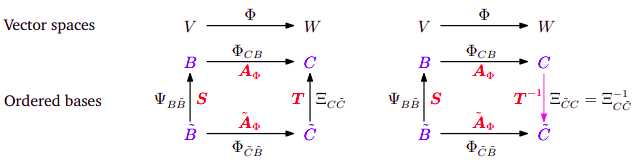
\includegraphics[
        width=\linewidth, 
        height=4cm,
        keepaspectratio,
    ]{images/maths-for-ml/basis-change.png}
    \caption*{
        For a homomorphism $\Phi  : V \to  W$ and ordered bases $B, \tilde{B}$ of $V$ and $C, \tilde{C}$ of $W$ (marked in \textcolor{blue}{blue}), we can express the mapping $\Phi _{\tilde{C} \tilde{B}}$ with respect to the bases $\tilde{B}, \tilde{C}$ equivalently as a composition of the homomorphisms $\Phi _{\tilde{C} \tilde{B}} = \Xi _{\tilde{C}C} \circ \Phi _{CB} \circ \Psi _{B\tilde{B}}$ with respect to the bases in the subscripts. 
        \\
        The corresponding transformation matrices are in \textcolor{red}{red}.
        \\
        We use $\Psi_{B\tilde{B}} = \text{id}_V$ and $\Xi _{C\tilde{C}} = \text{id}_W$ , i.e., the identity mappings that map vectors onto themselves, but with respect to a different basis.
        \hfill \cite{mfml/book/mml/Deisenroth-Faisal-Ong}
    }
\end{figure}


\begin{enumerate}
    \item \textbf{Theorem}: For a linear mapping $\Phi : V \to W$, ordered bases
    \hfill \cite{mfml/book/mml/Deisenroth-Faisal-Ong}
    \\
    .\hfill
    $
        B = (\bm{b}_1, \cdots , \bm{b}_n), \ 
        \tilde{B} = (\tilde{\bm{b}}_1, \cdots , \tilde{\bm{b}}_n)
    $
    \hfill \cite{mfml/book/mml/Deisenroth-Faisal-Ong}
    \\
    of $V$ and
    \hfill \cite{mfml/book/mml/Deisenroth-Faisal-Ong}
    \\
    .\hfill
    $
        C = (\bm{c}_1, \cdots , \bm{c}_n), \ 
        \tilde{C} = (\tilde{\bm{c}}_1, \cdots , \tilde{\bm{c}}_n)
    $
    \hfill \cite{mfml/book/mml/Deisenroth-Faisal-Ong}
    \\
    of $W$, and a transformation matrix $\bm{A}_\Phi$ of $\Phi$ with respect to $B$ and $C$, the corresponding transformation matrix $\tilde{\bm{A}} _\Phi$ with respect to the bases $\tilde{B}$ and $\tilde{C}$ is given as
    $
        \tilde{\bm{A}} \Phi = \bm{T}^{-1}\bm{A}_\Phi \bm{S}
    $.
    \hfill \cite{mfml/book/mml/Deisenroth-Faisal-Ong}
    \\
    Here, $\bm{S} \in \mathbb{R}^{n\times n}$ is the transformation matrix of $\text{id}_V$ that maps coordinates with respect to $\tilde{B}$ onto coordinates with respect to $B$, \ 
    and $\bm{T} \in \mathbb{R}^{m\times m}$ is the transformation matrix of $\text{id}_W$ that maps coordinates with respect to $\tilde{C}$ onto coordinates with respect to $C$.
    \hfill \cite{mfml/book/mml/Deisenroth-Faisal-Ong}

    \item \textbf{Proof}: we can write the vectors of the new basis $\tilde{B}$ of $V$ as a linear combination of the basis vectors of $B$, such that:
    \hfill \cite{mfml/book/mml/Deisenroth-Faisal-Ong}
    \\
    .\hfill
    $
        \tilde{\bm{b}}_j 
        = s_{1j} \bm{b}_1 + \cdots + s_{nj} \bm{b}_n 
        = \dsum^n _{i=1} s_{ij} \bm{b}_i 
        , j = 1, \cdots , n
    $
    \hfill \cite{mfml/book/mml/Deisenroth-Faisal-Ong}
    \\
    Similarly, we write the new basis vectors $\tilde{C}$ of $W$ as a linear combination of the basis vectors of $C$, which yields
    \hfill \cite{mfml/book/mml/Deisenroth-Faisal-Ong}
    \\
    .\hfill
    $
        \tilde{\bm{c}}_k 
        = t_{1k} \bm{c}_1 + \cdots + t_{mk} \bm{c}_m 
        = \dsum^m _{l=1} t_{lk} \bm{c}_l 
        , k = 1, \cdots , m
    $
    \hfill \cite{mfml/book/mml/Deisenroth-Faisal-Ong}
    \\
    We define $\bm{S} = ((s_{ij} )) \in \mathbb{R}^{n\times n}$ as the transformation matrix that maps coordinates with respect to $\tilde{B}$ onto coordinates with respect to $B$ and $\bm{T} = ((t_{lk})) \in R^{m\times m}$ as the transformation matrix that maps coordinates with respect to $\tilde{C}$ onto coordinates with respect to $C$. 
    In particular, the $j$-th column of $\bm{S}$ is the coordinate representation of $\tilde{\bm{b}}_j$ with respect to $B$ and the $k$-th column of $\bm{T}$ is the coordinate representation of $\tilde{\bm{c}}_k$ with respect to $C$. 
    Note that both $\bm{S}$ and $\bm{T}$ are regular.
    \hfill \cite{mfml/book/mml/Deisenroth-Faisal-Ong}
    \\
    We are going to look at $\Phi(\tilde{\bm{b}}_j )$ from two perspectives.
    \hfill \cite{mfml/book/mml/Deisenroth-Faisal-Ong}
    \begin{enumerate}
        \item Applying the mapping $\Phi$, we get that for all $j = 1, \cdots , n$
        \hfill \cite{mfml/book/mml/Deisenroth-Faisal-Ong}
        \\
        .\hfill
        $
            \Phi(\tilde{\bm{b}}_j )
            = \dsum^m_{k=1} \underset{\displaystyle \in W}{
                \underbrace{\tilde{a}_{kj} \textcolor{blue}{\tilde{\bm{c}}_k}}
            }
            = \dsum^m_{k=1} \tilde{a}_{kj} \textcolor{blue}{
                \dsum^m_{l=1} t_{lk} \bm{c}_l
            }
            = \dsum^m_{l=1} \dParenBrac{
                \textcolor{PineGreen}{\dsum^m_{k=1} t_{lk} \tilde{a}_{kj}} 
            }  \bm{c}_l
        $
        \hfill \cite{mfml/book/mml/Deisenroth-Faisal-Ong}
        \\
        where we first expressed the new basis vectors $\tilde{\bm{c}}_k \in W$ as linear combinations of the basis vectors $\bm{c}_l \in W$ and then swapped the order of summation.
        \hfill \cite{mfml/book/mml/Deisenroth-Faisal-Ong}


        \item when we express the $\tilde{\bm{b}}_j \in V$ as linear combinations of $\bm{b}_j \in V$ , we arrive at ($j = 1,\cdots, n$) :
        \hfill \cite{mfml/book/mml/Deisenroth-Faisal-Ong}
        \\
        .\hfill
        $
            \Phi (\tilde{\bm{b}}_j ) 
            = \Phi  \dParenBrac{ \textcolor{blue}{\dsum ^n _{i=1} s_{ij} \bm{b}_i}}
            = \dsum ^n _{i=1} s_{ij} \textcolor{red}{\Phi (\bm{b}_i)} 
            = \dsum^n _{i=1} s_{ij} \textcolor{red}{\dsum ^m _{l=1} a_{li} \bm{c}_l}
            = \dsum ^m _{l=1} \dParenBrac{ \textcolor{PineGreen}{\dsum^n _{i=1} s_{ij} a_{li}} } \bm{c}_l
        $
        \hfill \cite{mfml/book/mml/Deisenroth-Faisal-Ong}

        \item $
            \begin{aligned}
                \dsum^m_{k=1} t_{lk} \tilde{a}_{kj} = \dsum^n _{i=1} s_{ij} a_{li}
                \hspace{1cm}
                \Rightarrow 
                \bm{T} \tilde{\bm{A}}_\Phi = \bm{A}_\Phi \bm{S} 
                \in \mathbb{R}^{m\times n}
                \hspace{1cm}
                \Rightarrow 
                \tilde{\bm{A}}_\Phi = \bm{T}^{-1} \bm{A}_\Phi \bm{S}
            \end{aligned}
        $
        \hfill \cite{mfml/book/mml/Deisenroth-Faisal-Ong}        
    \end{enumerate}

    
\end{enumerate}






\subsection{Orthonormal Basis}


\begin{enumerate}
    \item 
\end{enumerate}




























\section{Linear Mappings}


\begin{figure}[H]
    \centering
    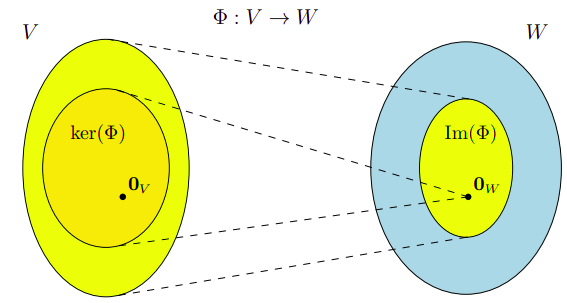
\includegraphics[
        width=\linewidth,
        height=4cm,
        keepaspectratio,
    ]{images/maths-for-ml/image-kernel-linear-mapping.png}
\end{figure}

\begin{enumerate}
    \item \textbf{Definition}: For vector spaces $V, W$, a mapping $\Phi : V \to W$ is called a linear mapping (or vector space homomorphism/ linear transformation) if
    \hfill \cite{mfml/book/mml/Deisenroth-Faisal-Ong}
    \\
    .\hfill
    $
        \forall \bm{x}, \bm{y} \in V \forall \lambda , \psi  \in \mathbb{R} : 
        \Phi(\lambda \bm{x} + \psi \bm{y}) = \lambda \Phi(\bm{x}) + \psi \Phi(\bm{y})
    $
    \hfill \cite{mfml/book/mml/Deisenroth-Faisal-Ong}

    \item we can represent linear mappings as matrices
    \hfill \cite{mfml/book/mml/Deisenroth-Faisal-Ong}

    \item For linear mappings $\Phi : V \to W$ and $\Psi : W \to X$, the mapping $\Psi \circ \Phi : V \to X$ is also linear.
    \hfill \cite{mfml/book/mml/Deisenroth-Faisal-Ong}

    \item If $\Phi : V \to W, \Psi : V \to W$ are linear, then $\Phi + \Psi$ and $\lambda\Phi, \lambda \in \mathbb{R}$, are linear, too.
    \hfill \cite{mfml/book/mml/Deisenroth-Faisal-Ong}
\end{enumerate}



\subsection{Matrix Representation of Linear Mappings}

\begin{enumerate}
    \item Any $n$-dimensional vector space is isomorphic to $\mathbb{R}^n$.
    \hfill \cite{mfml/book/mml/Deisenroth-Faisal-Ong}

    \item We consider a basis $\dCurlyBrac{\bm{b}_1, \cdots , \bm{b}_n}$ of an $n$-dimensional vector space $V$ .
    \hfill \cite{mfml/book/mml/Deisenroth-Faisal-Ong}
\end{enumerate}




\subsection{Image/Range \& Kernel/Null space}

\begin{enumerate}
    \item \textbf{Definition}: For $\Phi  : V \to W$, we define the image/range
    \hfill \cite{mfml/book/mml/Deisenroth-Faisal-Ong}
    \\
    .\hfill
    $
        \text{Im}(\Phi ) 
        := \Phi (V ) 
        = \dCurlyBrac{\bm{w} \in W|\exists \bm{v} \in V : \Phi (\bm{v}) = \bm{w}}
    $
    \hfill \cite{mfml/book/mml/Deisenroth-Faisal-Ong}

    \item \textbf{Definition}: For $\Phi  : V \to W$, we define the kernel/null space
    \hfill \cite{mfml/book/mml/Deisenroth-Faisal-Ong}
    \\
    .\hfill
    $
        \ker(\Phi ) 
        := \Phi ^{-1} (\bm{0}_W ) 
        = \dCurlyBrac{\bm{v} \in V : \Phi (\bm{v}) = \bm{0}_W }
    $
    \hfill \cite{mfml/book/mml/Deisenroth-Faisal-Ong}


    \item We also call $V$ and $W$ also the \textbf{domain} and \textbf{codomain} of $\Phi$, respectively.
    \hfill \cite{mfml/book/mml/Deisenroth-Faisal-Ong}

    \item The image is the set of vectors $\bm{w} \in W$ that can be “reached” by $\Phi$ from any vector in $V$ .
    \hfill \cite{mfml/book/mml/Deisenroth-Faisal-Ong}

    \item Intuitively, the kernel is the set of vectors $\bm{v} \in V$ that $\Phi$ maps onto the neutral element $\bm{0}_W \in W$.
    \hfill \cite{mfml/book/mml/Deisenroth-Faisal-Ong}

    \item It always holds that $\Phi(\bm{0}_V ) = \bm{0}_W$ and, therefore, $\bm{0}_V \in \ker(\Phi)$. 
    In particular, the null space is never empty.
    \hfill \cite{mfml/book/mml/Deisenroth-Faisal-Ong}

    \item $Im(\Phi) \subseteq W$ is a subspace of $W$, and $\ker(\Phi) \subseteq V$ is a subspace of $V$ .
    \hfill \cite{mfml/book/mml/Deisenroth-Faisal-Ong}

    \item $\Phi$ is injective (one-to-one) if and only if $\ker(\Phi) = \dCurlyBrac{\bm{0}}$.
    \hfill \cite{mfml/book/mml/Deisenroth-Faisal-Ong}

    \item \textbf{Rank-Nullity Theorem}: For vector spaces $V, W$ and a linear mapping $\Phi : V \to W$ it holds that $\dim(\ker(\Phi)) + \dim(\text{Im}(\Phi)) = \dim(V )$.
    \hfill \cite{mfml/book/mml/Deisenroth-Faisal-Ong}
    \begin{enumerate}
        \item The rank-nullity theorem is also referred to as the \textbf{fundamental theorem of linear mappings}
        \hfill \cite{mfml/book/mml/Deisenroth-Faisal-Ong}

        \item If $\dim(\text{Im}(\Phi )) < \dim(V )$, then $\ker(\Phi)$ is non-trivial, i.e., the kernel contains more than $\bm{0}_V$ and $\dim(\ker(\Phi)) \geq 1$.
        \hfill \cite{mfml/book/mml/Deisenroth-Faisal-Ong}

        \item If $\bm{A}_\Phi $ is the transformation matrix of $\Phi$  with respect to an ordered basis and $\dim(\text{Im}(\Phi )) < \dim(V )$, then the system of linear equations $\bm{A}_\Phi \bm{x} = \bm{0}$ has infinitely many solutions.
        \hfill \cite{mfml/book/mml/Deisenroth-Faisal-Ong}

        \item If $\dim(V ) = \dim(W)$, then the following three-way equivalence holds:
        \begin{enumerate}
            \item $\Phi$ is injective
            \item $\Phi$ is surjective
            \item $\Phi$ is bijective
        \end{enumerate}
        since $\text{Im}(\Phi) \subseteq W$.
    \end{enumerate}
\end{enumerate}













\section{Affine Mapping}

\begin{enumerate}
    \item \textbf{Definition}: For two vector spaces $V, W$, a linear mapping $\Phi : V \to W$, and $\bm{a} \in W$, the mapping:
    \hfill \cite{mfml/book/mml/Deisenroth-Faisal-Ong}
    \\
    .\hfill
    $ \phi : V \to W $ such that $ \bm{x} \mapsto \bm{a} + \Phi(\bm{x}) $
    \hfill \cite{mfml/book/mml/Deisenroth-Faisal-Ong}
    \\
    is an affine mapping from $V$ to $W$. 
    The vector a is called the \textbf{translation vector} of $\phi$.
    \hfill \cite{mfml/book/mml/Deisenroth-Faisal-Ong}

    \item Every affine mapping $\phi  : V \to W$ is also the composition of a linear mapping $\phi  : V \to W$ and a translation $\tau : W \to W$ in $W$, such that $\phi  = \tau \circ \phi $. 
    The mappings $\phi $ and $\tau$ are uniquely determined.
    \hfill \cite{mfml/book/mml/Deisenroth-Faisal-Ong}

    \item The composition $\phi ^\prime \circ \phi $ of affine mappings $\phi  : V \to W, \phi ^\prime: W \to X$ is affine.
    \hfill \cite{mfml/book/mml/Deisenroth-Faisal-Ong}

    \item Affine mappings keep the geometric structure invariant. 
    They also preserve the dimension and parallelism.
    \hfill \cite{mfml/book/mml/Deisenroth-Faisal-Ong}
\end{enumerate}



























\section{Injective, Surjective, Bijective Mappings}

\textbf{Definition}: Consider a mapping $\Phi : \mathcal{V} \to \mathcal{W}$, where $\mathcal{V}, \mathcal{W}$ can be arbitrary sets. 
Then $\Phi$ is called:
\hfill \cite{mfml/book/mml/Deisenroth-Faisal-Ong}

\begin{enumerate}
    \item \textbf{Injective} if $\forall \bm{x}, \bm{y} \in \mathcal{V} : \Phi(\bm{x}) = \Phi(\bm{y}) \Rightarrow \bm{x} = \bm{y}$
    \hfill \cite{mfml/book/mml/Deisenroth-Faisal-Ong}

    \item \textbf{Surjective} if $\Phi(\mathcal{V}) = \mathcal{W}$
    \hfill \cite{mfml/book/mml/Deisenroth-Faisal-Ong}
    \begin{enumerate}
        \item If $\Phi$ is surjective, then every element in $\mathcal{W}$ can be “reached” from $\mathcal{V}$ using $\Phi$.
        \hfill \cite{mfml/book/mml/Deisenroth-Faisal-Ong}
    \end{enumerate}
    
    \item \textbf{Bijective} if it is injective and surjective
    \hfill \cite{mfml/book/mml/Deisenroth-Faisal-Ong}
    \begin{enumerate}
        \item A bijective $\Phi$ can be “undone”, i.e., there exists a mapping $\Psi : W \to V$ so that $\Psi \circ \Phi(\bm{x}) = \bm{x}$.
        \hfill \cite{mfml/book/mml/Deisenroth-Faisal-Ong}

        \item This mapping $\Psi$ is then called the inverse of $\Phi$ and normally denoted by $\Phi^{-1}$.
        \hfill \cite{mfml/book/mml/Deisenroth-Faisal-Ong}
    \end{enumerate}    

\end{enumerate}


















\section{Special cases of Linear mappings}

\textbf{Definition}: Consider a mapping $\Phi : V \to W$, where $V, W$ can be arbitrary vector spaces. 
Then:
\hfill \cite{mfml/book/mml/Deisenroth-Faisal-Ong}

\begin{enumerate}
    \item \textbf{Isomorphism}: $\Phi : V \to W$ linear and bijective
    \hfill \cite{mfml/book/mml/Deisenroth-Faisal-Ong}
    \begin{enumerate}
        \item \textbf{Theorem}: Finite-dimensional vector spaces $V$ and $W$ are isomorphic if and only if $\dim(V ) = \dim(W)$.
        \hfill \cite{mfml/book/mml/Deisenroth-Faisal-Ong}

        \item there exists a linear, bijective mapping between two vector spaces of the same dimension.
        Intuitively, this means that vector spaces of the same dimension are kind of the same thing, as they can be transformed into each other without incurring any loss.
        \hfill \cite{mfml/book/mml/Deisenroth-Faisal-Ong}

        \item It gives the justification to treat $\mathbb{R}^{m\times n}$ (the vector space of $m \times n$-matrices) and $\mathbb{R}^{mn}$ (the vector space of vectors of length $mn$) the same, as their dimensions are $mn$, and there exists a linear, bijective mapping that transforms one into the other.
        \hfill \cite{mfml/book/mml/Deisenroth-Faisal-Ong}

        \item If $\Phi : V \to W$ is an isomorphism, then $\Phi ^{-1} : W \to V$ is an isomorphism, too.
        \hfill \cite{mfml/book/mml/Deisenroth-Faisal-Ong}
    \end{enumerate}

    \item \textbf{Endomorphism}: $\Phi : V \to V$ linear
    \hfill \cite{mfml/book/mml/Deisenroth-Faisal-Ong}

    \item \textbf{Automorphism}: $\Phi : V \to V$ linear and bijective
    \hfill \cite{mfml/book/mml/Deisenroth-Faisal-Ong}

    \item \textbf{identity mapping} or \textbf{identity automorphism}: $id_V : V \to V , \bm{x} \mapsto \bm{x}$
    \hfill \cite{mfml/book/mml/Deisenroth-Faisal-Ong}
\end{enumerate}



















\section{Transformation Matrix ( $A_\Phi$ )}

\begin{enumerate}
    \item \textbf{Definition}: Consider vector spaces $V$, $W$ with corresponding (ordered) bases $B = (\bm{b}_1, \cdots , \bm{b}_n)$ and $C = (\bm{c}_1, \cdots , \bm{c}_m)$. 
    Moreover, we consider a linear mapping $\Phi : V \to W$. 
    For $j \in \dCurlyBrac{1, \cdots , n}$,
    \hfill \cite{mfml/book/mml/Deisenroth-Faisal-Ong}
    \\
    .\hfill
    $
        \Phi(\bm{b}_j ) = \alpha _{1j} \bm{c}_1 + \cdots + \alpha _{mj} \bm{c}_m 
        = \dsum^m_{i=1} \alpha _{ij} \bm{c}_i
    $
    \hfill \cite{mfml/book/mml/Deisenroth-Faisal-Ong}
    \\
    is the unique representation of $\Phi(\bm{b}_j )$ with respect to $C$. 
    Then, we call the $m \times n$-matrix $\bm{A}_\Phi$, whose elements are given by $\bm{A}_\Phi(i, j) = \alpha_{ij}$ the transformation matrix of $\Phi$ (with respect to the ordered bases $B$ of $V$ and $C$ of $W$  ).
    \hfill \cite{mfml/book/mml/Deisenroth-Faisal-Ong}

    \item The transformation matrix can be used to map coordinates with respect to an ordered basis in $V$ to coordinates with respect to an ordered basis in $W$.
    \hfill \cite{mfml/book/mml/Deisenroth-Faisal-Ong}

    \item Consider vector spaces $V, W, X$. 
    We already know that for linear mappings $\Phi  : V \to  W$ and $\Psi : W \to  X$ the mapping $\Psi \circ \Phi  : V \to  X$ is also linear. 
    With transformation matrices $\bm{A}_\Phi$  and $\bm{A}_\Psi$ of the corresponding mappings, the overall transformation matrix is $\bm{A}_{\Psi\circ\Phi}  = \bm{A}_\Psi \bm{A}_\Phi$ .
    \hfill \cite{mfml/book/mml/Deisenroth-Faisal-Ong}

    \item 
    $\bm{A}_\Phi$  is the transformation matrix of a linear mapping $\Phi _{CB} : V \to  W$ with respect to the bases $B, C$.
    \hfill \cite{mfml/book/mml/Deisenroth-Faisal-Ong}
    \\[0.2cm]
    $\tilde{\bm{A}}_\Phi$  is the transformation matrix of the linear mapping $\Phi_ {\tilde{C}\tilde{B}} : V \to  W$ with respect to the bases $\tilde{B}, \tilde{C}$.
    \hfill \cite{mfml/book/mml/Deisenroth-Faisal-Ong}
    \\[0.2cm]
    $\bm{S}$ is the transformation matrix of a linear mapping $\Psi _{B\tilde{B}} : V \to  V$ (automorphism) that represents $\tilde{B}$ in terms of $B$. Normally, $\Psi  = \text{id}_V$ is the identity mapping in $V$ .
    \hfill \cite{mfml/book/mml/Deisenroth-Faisal-Ong}
    \\[0.2cm]
    $\bm{T}$ is the transformation matrix of a linear mapping $\Xi _{C\tilde{C}} : W \to  W$ (automorphism) that represents $\tilde{C}$ in terms of $C$. Normally, $\Xi  = \text{id}_W$ is the identity mapping in $W$.
    \hfill \cite{mfml/book/mml/Deisenroth-Faisal-Ong}
    \\[0.2cm]
    If we (informally) write down the transformations just in terms of bases, then $\bm{A}_\Phi  : B \to  C$, $\tilde{\bm{A}}_\Phi  : \tilde{B} \to  \tilde{C}$, $\bm{S} : \tilde{B} \to  B$, $\bm{T} : \tilde{C} \to  C$ and $\bm{T}^{-1} : C \to  \bm{C}$, and
    \hfill \cite{mfml/book/mml/Deisenroth-Faisal-Ong}
    \\[0.2cm]
    .\hfill
    $
        \tilde{B} \to  \tilde{C} = \textcolor{blue}{\tilde{B} \to  B} \textcolor{red}{\to  C} \to  \tilde{C} 
        \Rightarrow
        \tilde{\bm{A}}_\Phi  = \bm{T}^{-1} \textcolor{red}{\bm{A}_\Phi} \textcolor{blue}{\bm{S}}
    $
    \hfill \cite{mfml/book/mml/Deisenroth-Faisal-Ong}
    \\[0.2cm]
    Note that the execution order is from \textbf{right to left} because vectors are multiplied at the right-hand side so that 
    \hfill \cite{mfml/book/mml/Deisenroth-Faisal-Ong}
    \\[0.2cm]
    .\hfill
    $\bm{x} \mapsto  \bm{Sx} \mapsto  \bm{A}_\Phi (\bm{Sx}) \mapsto \bm{T}^{-1}(\bm{A}_\Phi (\bm{Sx})) = \tilde{\bm{A}}_\Phi \bm{x}$.
    \hfill \cite{mfml/book/mml/Deisenroth-Faisal-Ong}

    \item  Orthogonal matrices define transformations that are rotations (with the possibility of flips).
    \hfill \cite{mfml/book/mml/Deisenroth-Faisal-Ong}
\end{enumerate}






\section{Coordinates}

\begin{enumerate}
    \item Consider a vector space $V$ and an ordered basis $B = (\bm{b}_1, \cdots , \bm{b}_n)$ of $V$ . 
    For any $\bm{x} \in V$ we obtain a unique representation (linear combination):
    \hfill \cite{mfml/book/mml/Deisenroth-Faisal-Ong}
    \\
    .\hfill
    $
        \bm{x} = \alpha_1 \bm{b}_1 + \cdots + \alpha_n \bm{b}_n
    $
    \hfill \cite{mfml/book/mml/Deisenroth-Faisal-Ong}
    \\
    of $\bm{x}$ with respect to $B$. 
    Then $\alpha_1, \cdots , \alpha_n$ are the coordinates of $\bm{x}$ with respect to $B$, and the vector:
    \hfill \cite{mfml/book/mml/Deisenroth-Faisal-Ong}
    \\
    .\hfill
    $
        \bm{\alpha} = \begin{bmatrix}
            \alpha_1 \\
            \vdots \\
            \alpha_n
        \end{bmatrix}
        \in \mathbb{R}^n
    $
    \hfill \cite{mfml/book/mml/Deisenroth-Faisal-Ong}
    \\
    is the \textbf{coordinate vector/ coordinate} representation of $\bm{x}$ with respect to the ordered basis $B$.
    \hfill \cite{mfml/book/mml/Deisenroth-Faisal-Ong}

    \item A basis effectively defines a coordinate system.
    \hfill \cite{mfml/book/mml/Deisenroth-Faisal-Ong}

    \item For an $n$-dimensional vector space $V$ and an ordered basis $B$ of $V$ , the mapping $\Phi : \mathbb{R}^n \to V , \Phi(\bm{e}_i) = \bm{b}_i , i = 1, \cdots , n$, is linear, where $(\bm{e}_1, \cdots , \bm{e}_n)$ is the standard basis of $\mathbb{R}^n$.
    \hfill \cite{mfml/book/mml/Deisenroth-Faisal-Ong}

    \item The coordinates of $\Phi(\bm{b}_j )$ with respect to the ordered basis $C$ of $W$ are the $j$-th column of $\bm{A}_\Phi$.
    \hfill \cite{mfml/book/mml/Deisenroth-Faisal-Ong}
    \hfill \cite{mfml/book/mml/Deisenroth-Faisal-Ong}
    \begin{enumerate}
        \item Consider (finite-dimensional) vector spaces $V$, $W$ with ordered bases $B$, $C$ and a linear mapping $\Phi : V \to W$ with transformation matrix $\bm{A}_\Phi$.
        \hfill \cite{mfml/book/mml/Deisenroth-Faisal-Ong}

        \item If $\hat{\bm{x}}$ is the coordinate vector of $\bm{x} \in V$ with respect to $B$ and $\hat{\bm{y}}$ the coordinate vector of $\bm{y} = \Phi(\bm{x}) \in W$ with respect to $C$, then $\hat{\bm{y}} = \bm{A}_\Phi \hat{\bm{x}}$.
        \hfill \cite{mfml/book/mml/Deisenroth-Faisal-Ong}
    \end{enumerate}    
\end{enumerate}



























